\subsubsection{Monitoring}
Quando vedete una freccia circolare bisogna pensare al \textbf{PDCA} (Plan Do 
Check Act). Infatti, ormai tutti i progetti sono circolari. \emph{Kaizen} è 
una parola giapponese che vuol dire “miglioramento continuo”. Quando si vede 
che c’è un delta, ovvero uno scostamento tra valore atteso e valore ottenuto, 
si cerca di operare per migliorarlo. Una volta raggiunti gli obiettivi 
prefissati, come previsto dal \textbf{PDCA}, bisogna fissare dei nuovi 
obiettivi da raggiungere per migliorarsi continuamente.

\begin{itemize}
\item ME1: monitorare e valutare la performance dell'IT;
\item ME2: monitorare e valutare i controlli interni;
\item ME3: assicurarsi della conformità normativa;
\item ME4: fornire una governance per l'IT.
\end{itemize}

Sulla nuova normativa di privacy se l'azienda non intraprenderà le procedure 
adeguate per preservare la privacy, avrà delle multe fino al 5\% del fatturato 
e la possibilità di andare a processo.

\subsubsection{SSE-CMM: System Security Eng -- Capability Maturity Model}

Modelli di maturità. Questa categorizzazione si applica a tutto. Nata per 
l'ingegneria del Software.
La maturità è la capacità di governare i processi: se si riesce anche a 
mettere in pratica il miglioramento continuo si è a livelli alti.

Di conseguenza, gli investitori saranno più portati a investire in aziende che 
hanno un CMM alto rispetto a uno basso, in quanto quelle basse (dallo Stage 2 
in giù) sono legate al lato ``umano''. Essere a livelli alti è anche un 
vantaggio che si può portare sul mercato.

Grazie a questo è possibile mettere in piedi un sistema di miglioramento 
continuo.

\begin{figure}[h!]
        \begin{center}
                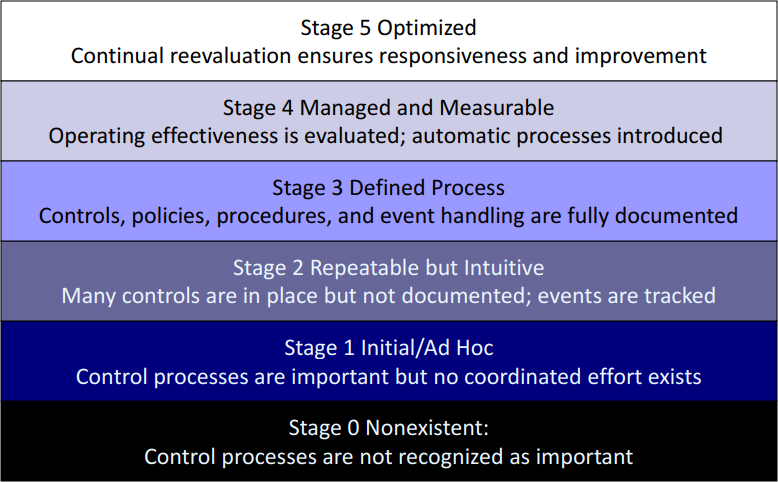
\includegraphics[scale=2.0]{res/img/maturity_level}
        \end{center}
        \caption{I 5 livelli del Capability Maturity Model (CMM).}
        \label{fig:cmm:levels}
\end{figure}

Se i controlli non sono documentati non si sa come possono essere migliorati, 
valutati, ecc\dots
\emph{I livelli sono molto importanti:} dal Livello 4 in su, 
l'automatizzazione dei processi di controllo permette un risparmio sul TCO 
(Total Cost of Ownership).



\subsubsection{Standard di sicurezza}

ISO 27001 e il COBIT sono gli standard di sicurezza di base. La \textit{gap 
analysis} (differenza tra dove vorremmo essere e dove siamo) ci aiuta a capire 
dove sono presenti le lacune da colmare.

\begin{figure}[h!]
        \begin{center}
                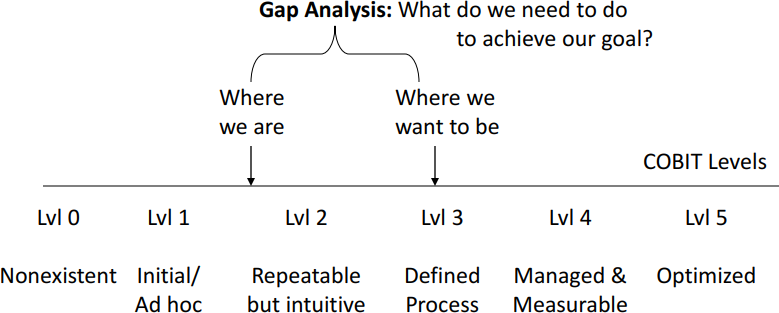
\includegraphics[scale=2.0]{res/img/security_standard}
        \end{center}
        \caption{I 5 livelli del Capability Maturity Model (CMM) e il
        loro rapporto con un programma di sicurezza.}
\end{figure}


\paragraph{Livello 0}

Al livello iniziale si è come un pompiere: si corre continuamente a destra e a 
sinistra per risolvere eventuali problemi.

\paragraph{Livello 1 - Esecuzione informale}

La progettazione della sicurezza è definita in maniera povera, i problemi di 
sicurezza sono trattati in maniera reattiva: si reagisce 
alla minaccia, portando prima o poi l'attacco a vincere. Non ci sono piani di 
contingenza\footnote{I piani di contingenza sono dei piani che dettano le 
azioni da compiere in caso si verificano delle situazioni d'emergenza.}. I 
budget, la qualità, le funzionalità e i progetti vengono schedulati \textit{ad 
hoc}. Non ci sono aree dei processi.

\paragraph{Livello 2 - Pianificato e Tracciato}

Le procedure vengono definite a livello di progetto. La definizione, 
pianificazione e le performance diventano de-facto standard da progetto a 
progetto. Gli eventi vengono tracciati. Le funzionalità comuni includono: 
pianificazione, disciplina, verifica e tracciamento delle performance.

\paragraph{Livello 3 - Ben definito}

I processi di sicurezza sono standardizzati all'interno dell'organizzazione e 
il personale viene addestrato per assicurarsi che abbia le conoscenze e le 
skill necessarie. In aggiunta, le misure vengono basate su un processo 
definito e gli audit tracciano le performance. Le funzionalità più comuni 
includono: definire un processo standard, eseguire il processo definito e 
coordinare le pratiche relative alla sicurezza.

\subparagraph*{Policy per la documentazione}

\begin{figure}[h!]
        \begin{center}
                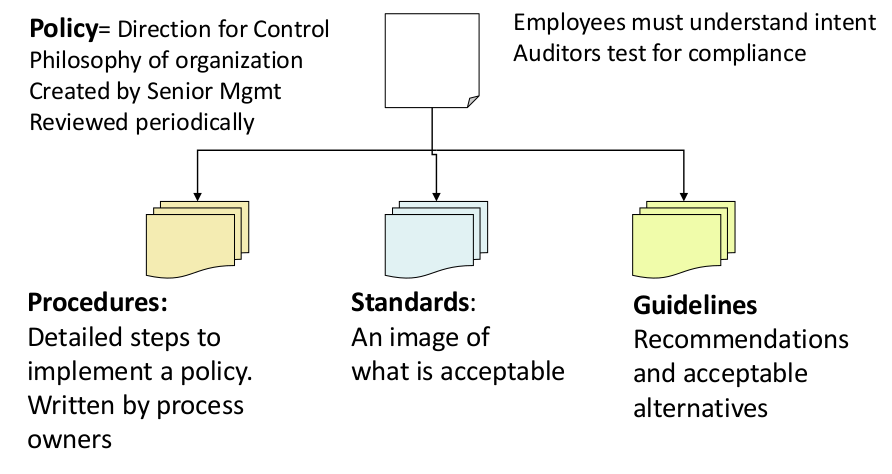
\includegraphics[scale=0.4]{res/img/documentation_policy}
        \end{center}
        \caption{Policy per la documentazione.}
\end{figure}

\subparagraph{Esempi di policy}

I \textbf{rischi} dovrebbero essere gestiti utilizzando dei controlli e delle 
contromisure appropriate per raggiungere dei livelli accettabili a dei costi 
accettabili. Il \textbf{monitoraggio} e le \textbf{metriche} dovrebbero essere 
implementate, gestite e mantenute per fornire una certezza continua che tutte 
le policy sulla sicurezza siano rispettate e i controlli oggettivi siano 
riscontrati. Le \textbf{capacità di risposta ad incidenti} sono implementate e 
gestite sufficientemente per garantire che gli incidenti non affliggano 
materialmente 
la capacità dell'organizzazione di continuare le proprie operazioni. 
La \textbf{business continuity} e il \textbf{recovery plan} dovrebbero essere 
sviluppate, mantenute e testate in modo che assicurino la capacità 
dell'organizzazione di proseguire con le proprie attività sotto tutte le 
condizioni.

Nota: una cattiva \textit{policy} fa riferimento alla tecnologia. Le 
\textit{policy} sono solamente linee guida.

\subparagraph{Policy, procedure e standard}

\subsubparagraph*{Obiettivo di una policy:} descrive \textit{cosa} deve essere 
soddisfatto.

\subsubparagraph*{Controllo della policy:} tecniche per raggiungere 
l'obiettivo, suddivise in
\begin{itemize}
\item \textbf{Procedure:} definiscono come la policy deve essere perseguita;
\item \textbf{Standard:} regola, metrica o vincolo specifico che implementa la 
policy.
\end{itemize}

\subparagraph{Definizioni della qualità}

\subsubparagraph*{Quality assurance:} assicurarsi che tutto lo staff stia 
seguendo i processi della qualità definiti.

\subsubparagraph*{Controllo della qualità:} condurre test per validare che il 
software è privo di difetti e corrisponde alle aspettative dell'utente.

\paragraph{Livello 4 - Metriche}

Esistono degli obiettivi misurabili per la qualità della sicurezza, le misure 
sono correlate agli obiettivi del business dell'organizzazione. Le 
funzionalità comuni includono: stabilire degli obiettivi misurabili di qualità 
e una gestione oggettiva delle performance (SLA).
È tutto scritto e documentato: sono presenti politiche, 
procedure, standard e linee guida.

\subparagraph{Metriche}

Le metriche permettono ad auditor differenti di attestare che i programmi per 
la sicurezza vengono attuati. Monitorare il raggiungimento di controlli 
oggettivi è più importante che perfezionare le procedure di sicurezza.

Senza metriche quantitative si lascia spazio alla soggettività.

\begin{figure}[h!]
        \begin{center}
                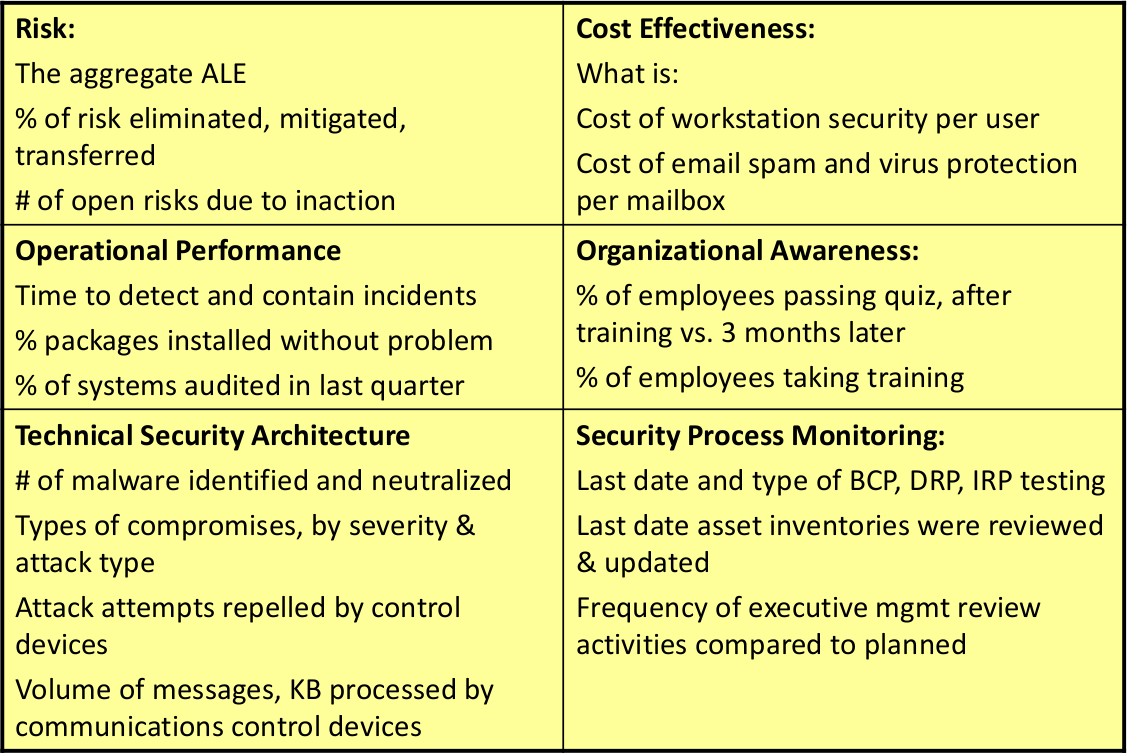
\includegraphics[scale=1.5]{res/img/metriche}
        \end{center}
        \caption{Esempi di metriche per un'azienda.}    
\end{figure}

\subsubparagraph*{Metriche operazionali}

Le metriche di tipo operazionale includono metriche su come eseguire 
un corretto \textit{patching} dei sistemi.

Confrontare le metriche con quelle di altre aziende permette di capire quanto 
siamo un possibile \textit{target} per gli attaccanti.

\subsubparagraph*{Metriche di tipo strategico}

Sono i piani legati al rischio, come il \textit{disaster recovery}.
Il rapporto di audit è una metrica importantissima perché fa capire come 
lavora l'azienda e l'auditor.

\subsubparagraph*{Compliance interna}

La conformità (\textit{compliance}) assicura la conformità con le policy 
organizzative. Compliance e errore interno sono dati importanti perché 
fanno capire all'azienda quanto è allineata con gli obiettivi strategici che 
si è prefissata.


\paragraph{Livello 5 - Miglioramento continuo}

Il miglioramento continuo parte dalle misure e dagli eventi sulla sicurezza.
Vengono valutate nuove tecnologie e nuovi processi. Le funzionalità comuni 
includono: miglioramento delle capacità organizzative e della efficacia dei 
processi (ROI).

Prima avere un cambio tecnologico di fondo è raro, oggi avviene ogni 3 anni. 
Chi prende la tecnologia e la incorpora si prende la fetta di mercato.

Le grandi società fanno \textit{scouting} di nuove tecnologie. Il vantaggio di 
essere un'azienda piccola è che si può essere aggressivi e investire, aiutando 
il movimento economico. Questo ci dice che aziende come Google non ci 
saranno per sempre. Non si è ancora capito a dove possa portare il cambiamento
tecnologico. Un'altra area importante è l'intelligenza artificiale legata 
alla sicurezza.


\subsubsection{Esercizi}

Gli esercizi sono disponibili in \ref{esSM:COBIT}

\chapter{Policy and Governance}
\label{PG}

\section{Governance}

\textbf{Corporate governance:} è la leadership da parte dei direttori 
aziendali nel creare e presentare il valore agli stakeholders.\\
\newline
\textbf{IT governance:} si assicura del corretto allineamento dell'IT con gli 
obiettivi aziendali.



\section{Strategic Planning Process}
\label{PG:SPP}

Oggi come oggi una \textbf{pianificazione strategica} nell'IT è in 3 anni, in 
quanto tra 5 anni nessuno sa cosa ci sarà. Quindi la lunghezza dei piani si è 
accorciata, specialmente nel settore informatico in quanto la pressione 
tecnologica è altissima. Questa pianificazione è destinata ad accorciarsi 
grazie all'intelligenza artificiale, che aiuterà gli umani a prendere 
decisioni. La \textbf{pianificazione tattica} dura un anno permette 
all'organizzazione di muoversi verso gli obiettivi strategici, mentre la 
\textbf{pianificazione operazionale} definisce piani dettagliati o tecnici.

\begin{figure}[H]
        \begin{center}
                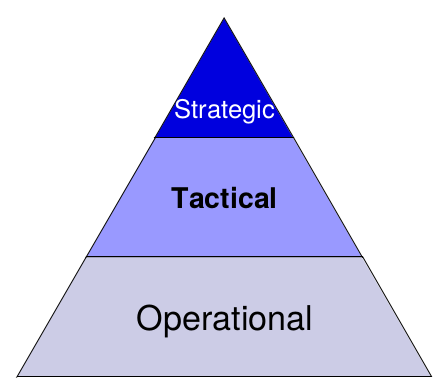
\includegraphics[scale=0.4]{res/img/planning_process}
        \end{center}
        \caption{Piramide dei differenti tipi di pianificazione.}    
\end{figure}

